%\documentclass[twocolumn,showpacs,preprintnumbers,amsmath,amssymb, floatfix]{revtex4}
\documentclass[aps,prb,preprint,preprintnumbers,amsmath,amssymb,floatfix,superscriptaddress]{revtex4}
%\documentclass[aps,prb,twocolumn,superscriptaddress,preprintnumbers,amsmath,amssymb,floatfix]{revtex4}

\usepackage{graphicx}
\usepackage{epstopdf}
\usepackage{ifthen}
\usepackage{dcolumn}
\usepackage{bm}
\usepackage{multirow}
\usepackage{booktabs}
\usepackage{amsbsy}
\usepackage{amsmath}
\usepackage{amssymb}
\usepackage{subfigure}
\usepackage{booktabs}
\usepackage{verbatim}

\graphicspath{
{/Users/mullspace/Dropbox/git/plots.nogit/images/}
{/home/schuberm/Dropbox/git/plots.nogit/images/}
{/home/mullspace/Dropbox/git/plots.nogit/images/}
}

%--------------------------------------------------------------------------
%DEFINE COMMANDS
%--------------------------------------------------------------------------
\newcommand{\EXP}[1]{\exp\mspace{-5.0mu}\left[#1\right]\mspace{-3.0mu}}

\newcommand{\SUM}[2]{\ifthenelse{\equal{#1}{0}}{\sum_{
\alpha_{#2},b_{#2},l_{#2}}^{3,n,N}} {\ifthenelse{\equal{#1}{1}}{\sum_{
\alpha_{#2},b_{#2}}^{3,n}}{\sum_{\pmb{\kappa}#2,\nu#2}^{N,3n}}}}

\newcommand{\ab}[2]{\mspace{-4.0mu}\left(\mspace{-8.0mu}
\begin{smallmatrix}&\ifthenelse{\equal{#1}{}}{a}{#1} \\&\ifthenelse
{\equal{#2}{}}{b}{#2}\end{smallmatrix}\mspace{-3.0mu}\right)}

\newcommand{\kvba}{\mspace{-4.0mu}\left(\mspace{-8.0mu}
\begin{smallmatrix} &\pmb{\kappa} &b \\ &\nu &\alpha\end{smallmatrix}
\mspace{-3.0mu}\right)}

\newcommand{\kvbap}{\mspace{-4.0mu}\left(\mspace{-8.0mu}
\begin{smallmatrix} &\pmb{\kappa}' &b \\ &\nu' &\alpha\end{smallmatrix}
\mspace{-3.0mu}\right)}

\newcommand{\kvt}{\mspace{-4.0mu}\left(\mspace{-8.0mu}
\begin{smallmatrix}&\pmb{\kappa} \\&\nu\end{smallmatrix}
\mspace{-2.0mu},t\right)}

\newcommand{\kvw}{\mspace{-4.0mu}\left(\mspace{-8.0mu}
\begin{smallmatrix}&\pmb{\kappa} \\&\nu\end{smallmatrix}
\mspace{-2.0mu},\omega\right)}

\newcommand{\kv}{\mspace{-4.0mu}\left(\mspace{-8.0mu}
\begin{smallmatrix}&\pmb{\kappa} \\&\nu\end{smallmatrix}
\mspace{-3.0mu}\right)}

\newcommand{\kvp}{\mspace{-4.0mu}\left(\mspace{-8.0mu}
\begin{smallmatrix}&\pmb{\kappa'} \\&\nu'\end{smallmatrix}
\mspace{-3.0mu}\right)}

\newcommand{\kw}{\mspace{-4.0mu}\left(\mspace{-8.0mu}
\begin{smallmatrix}&\pmb{\kappa} \\&\omega\end{smallmatrix}
\mspace{-3.0mu}\right)}

\newcommand{\lbt}{\mspace{-4.0mu}\left(\mspace{-8.0mu}
\begin{smallmatrix}&l \\&b\end{smallmatrix}\mspace{-2.0mu};t\right)}
%--------------------------------------------------------------------------
%END COMMANDS
%--------------------------------------------------------------------------
%--------------------------------------------------------------------------
\begin{document}

\title{Disruption of Superlattice Phonons through Interfacial Mixing}
\author{Samuel C. Huberman}
\affiliation{Department of Mechanical \& Industrial Engineering, University of Toronto, 
Toronto, Ontario M5S 3G8, Canada}
\author{Jason M. Larkin}
\affiliation{Department of Mechanical Engineering\\Carnegie Mellon University\\Pittsburgh, PA 15213}
\author{Alan J. H. McGaughey}
%\email{mcgaughey@cmu.edu}
\affiliation{Department of Mechanical Engineering\\Carnegie Mellon University\\Pittsburgh, PA 15213}
\author{Cristina H. Amon}
\affiliation{Department of Mechanical \& Industrial Engineering, University of Toronto, 
Toronto, Ontario M5S 3G8, Canada}
\affiliation{Department of Mechanical Engineering\\Carnegie Mellon University\\Pittsburgh, PA 15213}

\date{\today}% It is always \today, today,
             %  but any date may be explicitly specified
\vspace{14mm}
  
\begin{abstract}

We use normal mode decomposition to obtain phonon properties from quasi-harmonic lattice dynamics calculations and classical molecular dynamics simulations in unstrained Lennard-Jones argon superlattices. The relaxation-time approximation of the Boltzmann transport equation is used to predict cross-plane and in-plane thermal conductivity for a range of superlattice period lengths. Debye scaling ($\omega^{-2}$) of phonon lifetimes is found a low frequencies and Rayleigh scaling ($\omega^{-4}$) for intermediate frequencies in superlattices with interfacial mixing. We find that interspecies mixing reduces a phonon's mean free path and for short-period superlattices, lifetimes below the Ioffe-Regel limit are observed.

\end{abstract}
\maketitle
%%%%
\section{Introduction}
Equilibrium \cite {PhysRevB.85.195302} and non-equilibrium \cite {PhysRevB.79.214307,PhysRevB.79.075316,PhysRevB.72.174302} studies of thermal studies have been performed on a variety of superlattices. Although these techniques make predictions about the trends of thermal conductivity, a mode by mode analysis is required to understand the effects of the secondary periodicity, which emerges by alternating layers of dissimilar atoms, upon phonon properties. Prior models relied upon the validity of bulk phonon properties\cite{walkauskas:2579,chen:220} and approximations of the specularity and diffusivity of the interfaces \cite {PhysRevB.57.14958} or lacked the computational power \cite {PhysRevB.70.081310}. Recent work used Density Functional Perturbation Theory to examine phonon properties in superlattice structures.\cite{Luckyanova16112012,doi:10.1021/nl202186y} Unlike these works, where the phonon properties for short period superlattices is used for larger period superlattices for computational reasons \cite{Luckyanova16112012, doi:10.1021/nl202186y} or interfacial mixing is neglected,\cite{doi:10.1021/nl202186y} we demonstrate the ability of normal mode decomposition (NMD) to predict the phonon properties in unstrained superlattices with perfect and mixed interfaces without making such approximations.
%%%
\section{Modeling Framework}
\subsection{Superlattice structure and interactions}\label{SEC:sl_struc}
%%%
The superlattices are built on a face centered cubic lattice,  with the two species differentiated by their masses ($m_1$, $m_3$). Atomic interactions are modeled using the Lennard - Jones potential for argon ($\epsilon= 1.67\times10^{-21}$ Joules and $\sigma= 3.4\times10^{-10}$ meters with a cutoff radius of $2.5\sigma$) for all possible pairwise interactions. This work uses dimensionless units unless otherwise noted ($E^*=E/\epsilon$, $T^*=Tk_B/\epsilon$, $\omega^*=\omega\sqrt{\sigma^2m_a/\epsilon}$, $k^*=km^{0.5}_a\sigma^2/(\epsilon^{0.5}k_B)$). The temperature is fixed at 20 Kelvin, with a lattice constant of $a=5.315 \AA$.\cite{alan}

Each superlattice is identified by the fundamental repeated unit of material, consisting of $N/2$ conventional face centered cubic unit cells of $m_1$ and $N/2$ unit cells of $m_3$ along the cross-plane direction, thus a $4\times4$ ($N\times N$) superlattices refers to a superlattice period of 4 ($N$) monolayers of $m_1$ and 4 ($N$) monolayers of $m_3$ as seen in Fig.~\ref{fig:md_domain}(a). No lattice strain was permitted as the effects have been studied elsewhere.\cite{PhysRevB.72.174302}  We consider $2\times2$, $4\times4$, $8\times8$ and $14\times14$ superlattices with a mass ratio ($m_3/m_1$) of 3, where $m_1$ is set to have the mass of argon. The Brouillin Zone (BZ) is a rectangular prism with boundaries at $2\pi/(2Na)$ in the cross-plane direction and $2\pi/a$ in the in-plane directions.
%%%
\begin{figure}[ht!]
\begin{center}
\scalebox{0.5}{ \includegraphics{4p_ai.eps}}
\renewcommand{\figure}{Fig.}
\caption{Atomic representation of a $4\times4$ superlattice for unmixed (top) and 80/20 interfacial mixing (bottom) cases. Green corresponds to $m_1$ and gray corresponds to $m_3$.}
\label{fig:md_domain}
\end{center}
\end{figure}
%%%

Following the approach of Landry and McGaughey,\cite{PhysRevB.79.075316} interfacial mixing is introduced by selecting the individual adjacent monolayers to an interface in the molecular dynamics computational cell and flipping the masses of randomly selected atoms until the desired concentrations were reached. For example, a 4x4 superlattice with interfacial mixing, which we designate as 80/20 in correspondence to the concentration of original/foreign species within the monolayer, is shown in Fig.~\ref{fig:md_domain}(b).

\subsection{Thermal conductivity predictions}
\subsubsection{Normal Mode Decomposition}
Like previous superlattice studies, \cite{Luckyanova16112012,doi:10.1021/nl202186y} the phonon Boltzmann Transport Equation (BTE) under the single mode relaxation time approximation,\cite{ziman_electrons_2001} is used to predict the thermal conductivity in the $i$th direction
%%%
\begin{equation}\label{EQ:M:conductivity}
\begin{split}
k_{vib,\mathbf{i}}=&\sum_{\pmb{\kappa},\nu} c_{ph}\kv
v^{2}_{g,\mathbf{i}}\kv \tau\kv.
\end{split}
\end{equation}
%%%
To obtain the required inputs for Eq.~(\ref{EQ:M:conductivity}), we follow the NMD procedure outlined by McGaughey\cite{PhysRevB.71.184305}, Turney \cite {PhysRevB.81.081411} and Larkin,\cite{jason_inpress} in which atomic velocities obtained from MD simulation are projected onto the eigenvectors obtained from harmonic lattice dynamics calculations. The MD simulations were conducted using the LAMMPS package.\cite{LAMMPS} The time step for molecular dynamics was set to 4.285 fs. The specific heat is set to be $c_{ph}\kv=k_B/V$, where $V$ is the volume of the MD domain, because the mechanics considered here are classical and obey Maxwell-Boltzmann statistics. As temperature increases, anharmonicity of the potential energy causes the specific heat to deviate from $k_B/V$. The effect is small for LJ systems at the studied temperature.\cite{jason_inpress} The unit cells for perfect superlattices, as depicted in Fig.~\ref{fig:md_domain}(a), are used as inputs for harmonic lattice dynamics (HLD) calculations, performed using the GULP package.\cite{GULP} The allowed wavevectors, $\pmb{\kappa}$, are determined by the number of repetitions of the unit cell used in the MD simulations
%%%
\begin{equation}\label{EQ:NMD:allowdkpt}
\pmb{\kappa} = \sum_{\alpha} \pmb{b}_{\alpha} \frac{n_{\alpha}}{N_{\alpha}},
\end{equation}
%%%
where $\pmb{b}_\alpha$ are the cubically orthogonal reciprocal lattice vectors and $ \frac{N_\alpha}{2} < n_\alpha \le \frac {N_\alpha}{2}$, where $n$ are integers and $N$ are constant even integers corresponding to the number of unit cells in the $\alpha$ direction so that the wavevectors are in the first BZ. Group velocities were calculated using finite differencing about a given frequency
%%%
\begin{equation}\label{EQ:NMD:vg}
\begin{split}
\pmb{v}_{g}\kv=\frac{\partial \omega \kv}{\partial \pmb{\kappa}}.
\end{split}
\end{equation}
%%%
The eigenvectors and the atomic velocities are are used as inputs to obtain the time series of the time derivative of the normal mode coordinate 
%%%
\begin{equation}\label{EQ:NMD:qdot}
\begin{split}
\dot{q}\kvt{}{}{}=&\SUM{0}{}\sqrt{\frac{m_b}{N}}\dot{u}_{\alpha}\lbt e^*\kvba\EXP{i\pmb{\kappa}\cdot\mathbf{r}_0\ab{l}{0}},
\end{split}
\end{equation}
%%%
where $\dot{u}_{\alpha}\lbt$ is the component of velocity of atom $b$ in the $l$ th unit cell in the $\alpha$ direction and $e^*\kvba$ denotes the complex conjugate of the $\alpha$ component for atom $b$ of the eigenvector for mode $\kv$. By taking the Fourier transform of the autocorrelation of the time derivative of the normal mode coordinate, the power spectrum is obtained \cite{dove_introduction_1993-3}
%%%
\begin{equation}\label{EQ:NMD:SED}
\begin{split}
T\kvw=&\lim_{\tau_0\rightarrow\infty}\frac{1}{2\tau_0}\left|\frac{1}{\sqrt{2\pi}}\int_{0}^{\tau_0}\dot{q}\kvt\exp(-i\omega t)dt\right|^2.
\end{split}
\end{equation}
%%% 
In analyzing the MD velocity data, the Fourier transform sampling window was set to $2^{16}$ time steps for all modes in the $2 \times 2$ and $4 \times 4$ superlattice and for modes with frequencies greater than one in the $8\times 8$ and $14 \times 14$ superlattices, with a total simulation time of $2^{20}$ for five independent MD simulations with different initial velocity seeds. The Fourier transform sampling window was set to $2^{20}$ and $2^{22}$ time steps for modes with frequencies less than one for $8\times 8$ and $14 \times 14$ superlattices, with total simulation time of $2^{20}$ and $2^{22}$ for ten independent MD simulations with different initial velocity seeds. The lag between velocity samples was $2^5$ time steps, which is sufficient to capture the dynamics of highest frequency modes. The power spectrum was averaged over all seeds and Fourier transform sampling windows. Further averaging was conducted by imposing the symmetry of the irreducible BZ. In accordance with anharmonic theory,\cite{maradudin_scattering_1962} the power spectrum can be approximated to be a Lorentzian, for cases where $\Gamma\kv \ll \omega\kv$, of the form 
%%%
\begin{equation}\label{EQ:NMD:LOR}
\begin{split}
T\kvw\approx&C_0\kv\frac{\Gamma\kv/\pi}{[\omega_0\kv-\omega]^2+\Gamma^2\kv},
\end{split}
\end{equation}
%%%
and thus fitting Eq.~(\ref{EQ:NMD:LOR}) to Eq.~(\ref{EQ:NMD:SED}) yields the phonon lifetime
%%%
\begin{equation}\label{EQ:lifetime}
\begin{split}
\tau\kv=&\frac{1}{2\Gamma\kv}.
\end{split}
\end{equation}
%%%
This spectral width corresponds to all possibles mechanisms of phonon interaction. Fitting of the power spectra to Eq.~(\ref{EQ:NMD:SED}) was done by only considering points within 3 orders of magnitude of the maximum value. A quantity of interest that can be measured experimentally \cite{Jon} is the phonon-phonon mean free path $\Lambda\kv$, defined as the distance travelled between scattering events \cite{ziman_electrons_2001}
%%%
\begin{equation}\label{EQ:M:phonon_mfp}
\begin{split}
\Lambda\kv &= |\pmb{v}_{g}\kv {}| \tau\kv.
\end{split}
\end{equation}
%%%
HLD was performed using unit cells for perfect superlattices and the same set of eigenvectors were used in the NMD analysis for both perfect and mixed cases. The effects of mixing are captured through the atomic velocities due to differences between perfect and mixed MD domains as described in Sec.~\ref{SEC:sl_struc}.

\subsubsection{Green-Kubo and Anharmonic Lattice Dynamics}
Green-Kubo (GK) simulations, previously validated against the non-equilibrium direct method,\cite {PhysRevB.79.075316} were performed on the the same molecular domain, for consistency, that was used in the NMD approach for both mixed and non mixed systems. Ten independent MD simulations were performed for each superlattice systems (perfect and mixed). The same time step that was used for the MD portion of the NMD is used for GK. The total  simulation length is $1\times 10^6$ timesteps, with a correlation window of $5\times 10^4$ timesteps for $2 \times 2$ and $4 \times 4$ superlattices and $1\times 10^5$ timesteps for $8 \times 8$ and $14 \times 14$. In order to minimize the error in the GK predictions, the converged value of the thermal conductivity was specified using the first avalanche method described by Chen et al. \cite{Chen20102392}

To provide additional context between thermal conductivity prediction methods, anharmonic lattice dynamics (ALD) was performed using the unit cells for unmixed systems described in Sec.~\ref{SEC:sl_struc}. Using the third order force constants of the LJ potential and perturbation theory, the phonon lifetimes are extracted and thermal conductivity is estimated using Eq.~(\ref{EQ:M:conductivity}). The details of ALD can be found elsewhere.\cite{PhysRevB.79.064301}

\section{Results}
\subsection{Dispersion and Power Spectra}

Phonon dispersion curves for the $4\times4$ superlattice is shown Fig.~\ref{fig:dispersion}(A-C). Dispersion curves for other superlattices show similar features, with more branches and decreasing length of the $[x,0,0]$ dimension of the BZ as the period length increases. Gaps emerge at the BZ boundaries as a consequence of branch folding.\cite{PhysRevB.38.1427,PhysRevB.60.2627} The flatness of the branches for $\omega > 15$ in Fig.~\ref{fig:dispersion}(A) suggest low group velocities and therefore small contribution of these modes to cross-plane thermal conductivity. Branches in Fig.~\ref{fig:dispersion}(B-C), on the other hand, behave non-linearly at most frequencies. The density of states shares the $\omega^2$ behavior at low frequencies with bulk $m_3$ (green line in Fig.~\ref{fig:dispersion}(D)). The inverse participation ratio, defined as $1/p\kv=\sum_{b,a}e\kvba^4$ and plotted in Fig.~\ref{fig:dispersion}(E), indicates that there is no spatial localization, which for completely delocalized modes is $p\approx card(\nu)$ and spatially localized is $p\approx 1$. \cite{PhysRevB.70.235214} The frequency dependence of the participation ratio and density of states was not found to vary with superlattice period length.
%%%
\renewcommand{\topfraction}{0.7}
\begin{figure*}%[H]
\begin{center}
\scalebox{1}{ \includegraphics{4p_dis_dos_pnum.eps}}
\renewcommand{\figure}{Fig.}
\caption{Dispersion (A,B,C), density of states (D) and inverse participation ratio (E) of a $4\times4$ superlattice. Red squares represent select modes for Fig.~\ref{fig:sed}.}
\label{fig:dispersion}
\end{center}
\end{figure*}
%%%

Selected sample power spectrums are shown in Fig.~\ref{fig:sed}. Note that while the peaks appear to be Lorentzian centered about single frequency, there are minor signatures at other frequencies. These signatures are attributed to the approximation that the normal mode of the harmonic system is equivalent to the normal mode of the anharmonic system. In the interfacial mixing cases, the intensity of the signatures becomes amplified, an indication of the mutual implications of disorder (random masses with linear springs) and anharmonicity (ordered masses with non-linear springs) upon phonon propagation. \cite{RevModPhys.53.175}  Modes around $\nu=20$ experience the largest disruptions for all dispersion directions, which may be a result of the large number of modes with similar frequencies, observed in the density of states shown in Fig.~\ref{fig:dispersion}(D) at $\omega=12$, available for these modes to interact and scatter with, as described in Allen-Feldmann theory.\cite{allen_thermal_1993,feldman_thermal_1993-1} Fitting a Lorentzian was deemed suitable for the mixed systems since the coefficient of determination value \cite{Cowpe20081066} for the most effected modes was about 0.9, but making the same assumption becomes increasingly questionable as the alloy limit is approached. \cite{jason2013vc}  Furthermore, the peaks may broaden to such a point where the condition $\Gamma\kv \ll \omega\kv$ is no longer satisfied, as is seen in the 60/40 case for mode 20 (Fig.~\ref{fig:sed}(b)). The superlattice dispersion allows one to capture the effects of the secondary periodicity upon group velocities and lifetimes. Interfacial mixing, however, disrupts this secondary periodicity and thus alters the dispersion relation. The wavevector for the perfect system is not guaranteed to  correspond to the same wavevector in the mixed system. In other words, the superlattice phonons which emerge from the secondary periodicity are effectively \textit{transformed} by the interfacial mixing. For the remainder of this work, the 80/20 system is used to discuss the effects of interfacial mixing upon phonon properties.
%%%
\renewcommand{\topfraction}{1.0}
\begin{figure*}%[t]
\begin{center}
\scalebox{1}{ 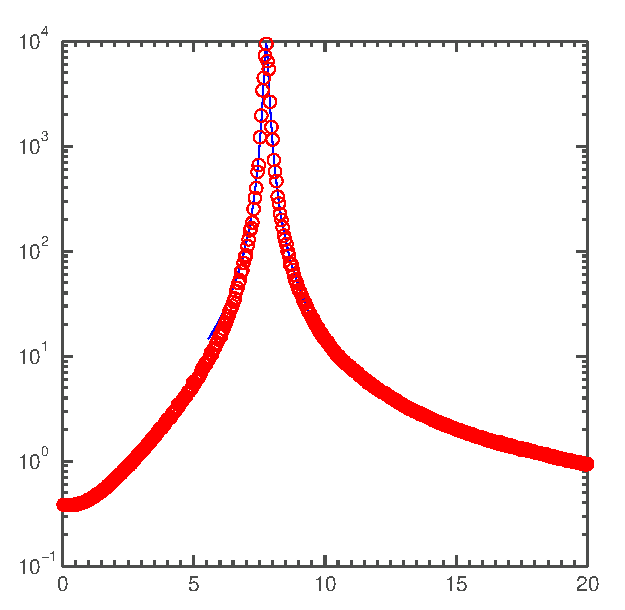
\includegraphics{sed.eps}}
\renewcommand{\figure}{Fig.}
\caption{(Colour online) Plots of the power spectrums for the selected modes as indicated by the red square markers in Fig.~\ref{fig:dispersion}(A-C). Dark blue corresponds to a superlattice without mixing, red corresponds to mixing of 80/20 and light blue corresponds to mixing of 60/40. Lifetimes calculated from the fitting of the Lorentzian functions (not shown) for the three systems are presented.}
\label{fig:sed}
\end{center}
\end{figure*}
%%%

%The consequences of using same set of eigenvectors were used in the NMD procedure for mixed and non-mixed $N\times N$ is observed in Figure~\ref{fig:sed}, where for modes at low and high frequency, the peaks remain well-defined, but some intermediate frequency modes become noticeably perturbed.  
%%%
%\begin{figure}%[H]
%\begin{center}
%\scalebox{0.8}{ 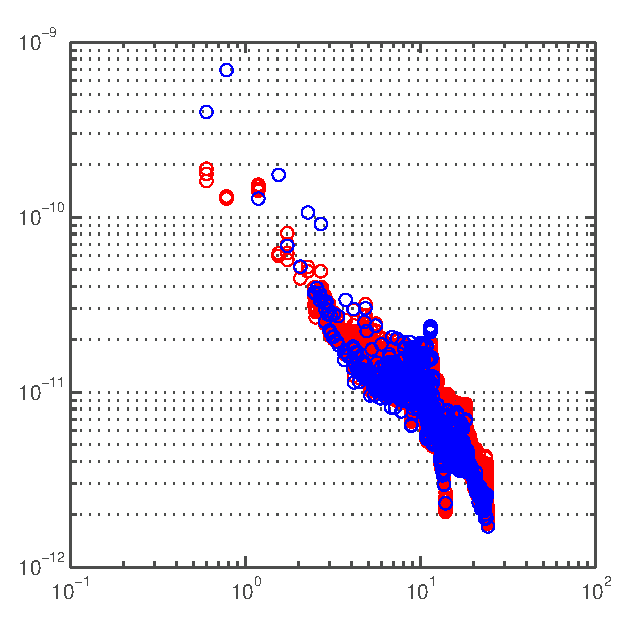
\includegraphics{/home/schuberm/Dropbox/git/plots.nogit/images/NMD_v_ALD.eps}}
%\renewcommand{\figure}{Fig.}
%\caption{Comparison between lifetimes from NMD and ALD in a $4\times4$ superlattice without interfacial mixing.}
%\label{FIG:NMD_v_ALD}
%\end{center}
%\end{figure}
%%%
%Confirm the validity of ALD

%Figure~\ref{FIG:NMD_v_ALD} shows no systematic bias between ALD and NMD for shorter lifetimes, with some systematic scatter at the longer lifetimes towards ALD. In general, ALD lifetimes are expected to be larger than NMD lifetimes because ALD neglects the contribution from $n$ order phonon processes\cite{PhysRevB.79.064301,esfarjani2011heat}, where $n$ is greater than 3.

\subsection{Lifetimes}

Phonon lifetime as a function of unshifted harmonic frequency is shown in Fig.~\ref{FIG:lifetime}. All superlattices exhibit $\omega^{-2}$ scaling at low frequencies, a consequence of the quadratic behaviour found in the density of states at these frequencies as seen in Fig.~\ref{fig:dispersion} (d).\cite{Klemens_Thermal_1951} For the larger period length superlattices ($8\times8$, $14\times14$), the non-mixed systems have two distinct $\omega^{-4}$ scalings which terminate at the maximum frequencies of the bulk systems of $m_1$ and $m_3$.

As interspecies mixing is introduced, there is a downwards shift in phonon lifetimes, particularly for the higher frequency modes of short period superlattices, shifting some modes below the Ioffe-Regel criterion. As the modes for a given superlattice have a plane wave structure, enforced by the harmonic solution of the lattice dynamics calculation, reaching the Ioffe-Regel criterion is an indication not of spatial localization but rather temporal localization and can thus be considered to be non-propagating delocalized modes.\cite{allen_thermal_1993} Similar trends in the variation of lifetimes with frequency, dipping below the Ioffe-Regel criterion at intermediate frequencies and recovering at higher frequencies, have recently been observed in alloys.\cite{jason2013vc} Spatial localization has been previously invoked to explain the thermal conductivity trends in superlattices \cite{PhysRevB.61.3091} but this is not the case for the systems studied here.

%%%
\renewcommand{\textfraction}{0.0}
\begin{figure}%[H]
\begin{center}
%\scalebox{1}{ \includegraphics{/Users/mullspace/Dropbox/git/plots.nogit/images/lifvomega.eps}}
\scalebox{1}{ \includegraphics{lifvomega.eps}}
\renewcommand{\figure}{Fig.}
\caption{Lifetimes for NMD-perfect (blue) and NMD-mixed (red) and Tamura theory (green). The black line corresponds to the Ioffe-Regel criterion, $2\pi\omega^{-1}$. The brown line corresponds to $\omega^{-2}$ scaling. The green line corresponds to $\omega^{-4}$ scaling. Vertical grey lines correspond to the maximum frequency observed in the bulk systems: for $m_1$, $\omega_1=24.7$ and for $m_3$, $\omega_3=14.3$. } 
\label{FIG:lifetime}
\end{center}
\end{figure}
%%%

A Rayleigh scattering scaling ($\omega^{-4}$) is observed at larger frequencies for smaller superlattice period lengths ($2\times2$, $4\times4$). The $\omega^{-4}$ scaling was theoretically predicted to dominate long wavelength modes due to elastic defect scattering.\cite{PhysRev.140.A1812,klemens_scattering_1955-3, klemens_thermal_1957-2} Because the determination of $\tau\kv$ does not distinguish between phonon scattering mechanisms, the $\omega^{-4}$ scaling diverges at low frequencies and is replaced by $\omega^{-2}$ scaling. 

Superlattice studies using DFPT and the BTE by Garg et al. suggest that interfactial disorder might explain the discrepancy between theoretical predictions and experimental measurements of cross-plane thermal conductivity. \cite{doi:10.1021/nl202186y}  The DFPT approach to calculating phonon properties, however, cannot explicitly determine the effects of mixing because, for one, the analysis is based in reciprocal space and as such imposes the same geometric mixing to all unit cells. Luckyanova et al. \cite{Luckyanova16112012} adopted Tamura elastic mass defect scattering theory \cite{tamura_isotope_1983} to modify the DFPT predicted lifetimes  ($\tau_{perfect}\kv$ ) through the Matthiesen rule
%%%
\begin{equation}\label{EQ:tau_eff}
\begin{split}
\frac{1}{\tau_{effective}\kv} = \frac{1}{\tau_{defect}\kv}+\frac{1}{\tau_{perfect}\kv} ,
\end{split}
\end{equation}
%%%
where, for the classical systems studied here, $\tau_{perfect}\kv$ is obtained from ALD and
%%%
\begin{equation}\label{EQ:tau_d}
\begin{split}
\frac{1}{\tau_{defect}\kv} = \frac{\pi}{2N_{uc}}\omega^2\kv 
\sum_{\pmb{\kappa'},\nu'} \delta( \omega\kv - \omega\kvp )\sum_{b} g_2(b) 
|e^*\kvbap \cdot e\kvba |^2 ,
\end{split}
\end{equation}
%%%
$N_{uc}$ is the total number of unit cells considered, and $g_2(b)$ is the coupling term which defines the strength of the mass disordering
%%%
\begin{equation}\label{EQ:g(b)}
\begin{split}
g_2(b) = \sum_\mu c_{\mu}(b)\left(1-\frac{m_{\mu}(b)}{\overline{m(b)}}\right)^2, 
\end{split}
\end{equation}
%%%
$c_\mu(b)$ is the concentration of the mixing, $m_\mu(b)$ is the mass of the $\mu$-th species and $\overline{m(b)}$ is the average mass for the $b$ atom in the unit cell. Given that there are two atom types in the superlattice unit cell, $\mu=1,3$, the atom $m_1$ can be considered to be a mass defect of the $m_3$ portion of the superlattice, with the reverse being equally true. $g_2(b)$ was set to be zero if atom $b$ remained unmixed (for atoms that do not reside within one monolayer of the interface) since $m_{\mu}(b)=\overline{m(b)}$. The delta function in Eq.~(\ref{EQ:tau_d}) is broadened into a Lorenztian of width on the order of the frequency level spacing imposed by the finite size of the systems.\cite{allen_thermal_1993}

Fig.~\ref{FIG:lifetime} shows general agreement between the lifetimes calculated using Eq.~(\ref{EQ:tau_eff}) and lifetimes obtained from NMD under the assumption that the eigenvectors of the unmixed systems are valid for the mixed systems; both resolve the $\omega^{-2}$ scaling at low frequencies and the general smearing at intermediate and larger frequencies. At larger frequencies, Tamura theory predicts lifetimes below the Ioffe-Regel limit for all superlattice period lengths.
%%%
\begin{comment}
\begin{table}
\begin{center}
\begin{tabular*}{\textwidth}{c@{\extracolsep{\fill}}ccccc}
\hline\hline\noalign{\smallskip}
&\multicolumn{3}{c}{$N\times N$ Superlattice} \\
\cline{2-5}\noalign{\smallskip}
\hspace{1cm} & $2\times2$ & $4\times4$ & $8\times8$ & $14\times14$  \\
\noalign{\smallskip}\hline\noalign{\smallskip}
%$\tau_{eff}$   & 0.51 $\pm$ 0.51 & 0.49 $\pm$ 0.59 &  0.33 $\pm$ 0.34& 0.21 $\pm$ 0.22 \\
%ALD   & 0 $\pm$ 0 & 0.11  $\pm$  0.14 &  0.09  $\pm$  0.07 & NA \\
RMSE $\sqrt{\frac{\sum_{\pmb{\kappa}\nu}(\tau_{eff}\kv-\tau_{mixed}\kv)^2}{n}}$ &0.65 & 1.21 & 2.09 & 5.42\\
Mean $\overline{\tau_{mixed}\kv}$ &1.37 & 1.93 & 2.74 & 3.40\\
Standard Deviation $\sigma[\tau_{mixed}\kv]$ &2.34 & 2.66 & 5.53 & 11.84\\
\noalign{\smallskip}\hline\hline
\end{tabular*}
\end{center}
\renewcommand{\table}{Table.}
\caption{The root-mean-square error between Tamura theory effective lifetimes and NMD mixed lifetimes. The mean and standard deviation of the NMD mixed lifetimes are provided for context. %ALD was not used for the 14x14 case due to the computational complexity of $\Omega (N_{uc}^4)$.}
}
\label{TB:taud}
\end{table}
\end{comment}
%%%

\subsection{Thermal Conductivity}

%%%
\begin{figure}%[H]
\begin{center}
\scalebox{1}{ \includegraphics{MFP_cp.eps}}
\renewcommand{\figure}{Fig.}
\caption{Phonon mean free path normalized by the period length contribution to the cross-plane thermal conductivity. From top to bottom $2\times2$, $4\times4$, $8\times8$ and $14\times14$ superlattices. Color corresponds to those used in Fig.~\ref{FIG:lifetime}. Average MFP is reported; subscripts correspond to the color of marker (b:blue, r:red, g:green).}
\label{FIG:MFP_cp}
\end{center}
\end{figure}
%%%

From Fig.~\ref{FIG:MFP_cp}, there is a clear reduction in the contribution to cross-plane thermal conductivity in perfect superlattices from modes with a MFP greater than the period length as period length increases. This trend is consistent with the theoretical predictions from Mahan that a minimum occurs as the transport behaviour shifts from a wave-regime to particle-regime.\cite{PhysRevLett.84.927,PhysRevB.56.10754} This same trend is observed in the contribution curves for the in-plane conductivity (not shown). The dimensional value of the peak MFP in perfect superlattices, for both in-plane and cross-plane, does not vary significantly as a function of period length. For short period superlattices ($2\times2$, $4\times4$ and $8\times8$), interfacial mixing shifts the average MFP towards the period length and reduces its respective contribution, indicative of the transition of thermal transport from superlattice phonons to thermal transport from phonons which may or may not map to those belonging to the perfect dispersion. This trend further supports the fact that superlattice phonons become disrupted by interfacial mixing, thereby diminishing the enhancing effects of the secondary periodicity upon cross-plane thermal conductivity. At large enough period lengths, the effect of interspecies mixing has a negligible effect on phonon MFP, as the corresponding lifetimes are less affected with increasing period length (Fig.~\ref{FIG:lifetime}) because of the decrease in the number of interfaces per unit of volume. \cite{PhysRevB.79.075316}

The linear extrapolation procedure used to predict bulk thermal conductivities \cite{PhysRevB.81.214305} was not used in previous superlattice studies \cite{doi:10.1021/nl202186y,Luckyanova16112012} and is not used here. Size effects were estimated by performing a convergence study. NMD predictions in both cross-plane and in-plane thermal conductivities varied by less than 10\% for systems with more than $N_x=8$ superlattice UCs along the cross-plane and $N_y=N_z=6$ UCs along the in-plane ($N_x=10$ was used for $2\times2$ to resolve the lifetime scalings). ALD was performed using $N_x=N_y=N_z=8$. Due to the time complexity of ALD ($O((N_i card(\nu)/3)^4)$) and NMD ($O(N_x  N_y N_z card(\nu))$), increasing the resolution of the Brillouin zone ($N_i$) was computational prohibitive. As a result of these size effects, the reported thermal conductivity predictions from NMD and ALD are presumed to carry, at a minimum, an uncertainty of 10\%.

A direct consequence of the finite size of the systems is the challenge in resolving longer wavelength modes because of the restricted resolution of the Brillouin zone enforced by the MD domain. This effect is observed in Fig.~\ref{FIG:MFP_cp}, where the finite number of resolved wavevectors leads to what would appear as noise in the contribution distribution at longer MFPs. This has been observed in other mode by mode analysis techniques, such as the real space force constant extraction from DFT method used by Esfarjani, where the limited resolution manifested in a stepwise behavior of thermal conductivity accumulation function.  \cite{PhysRevB.84.085204} The linear behavior of the dispersion near the gamma point and the $\omega^{-2}$ scaling of the lifetimes allowed for the contribution of these unresolved long-wavelength modes to be estimated. The complicated dispersion (Fig.~\ref{fig:dispersion}(A-C)) does not guarantee that such an approach is viable, as such, understanding size effects in superlattices warrants further work.

\begin{table}
\begin{center}
\begin{tabular*}{\textwidth}{c@{\extracolsep{\fill}}cccccc}
\hline\hline\noalign{\smallskip}
&&\multicolumn{4}{c}{$N\times N$ Superlattice} \\
\cline{3-6}\noalign{\smallskip}
\hspace{1cm} && $2\times2$ & $4\times4$ & $8\times8$ & $14\times14$  \\
\noalign{\smallskip}\hline\noalign{\smallskip}
\multirow{4}{*}{Perfect} &NMD & 0.29 & 0.24  & 0.32  & 0.39 \\
&GK & 0.25 $\pm$ 0.02 & 0.22 $\pm$ 0.04  &  0.29 $\pm$ 0.02  &  0.39 $\pm$ 0.03\\
&ALD & 0.25 &	0.26  &	0.32	 &0.44\\
&Thermal Circuit & 0.07  &  0.13  &  0.23  &  0.32\\
\noalign{\smallskip}\hline
\multirow{4}{*}{Mixed} &NMD &0.19 & 0.17 & 0.28 & 0.39\\
&GK  & 0.16 $\pm$ 0.01  &  0.18 $\pm$ 0.02 &  0.28 $\pm$ 0 &   0.45 $\pm$ 0.06\\
&Tamura (NMD) & 0.21 & 0.15 & 0.30 & 0.37\\
&Tamura (ALD) & 0.12 & 0.19 & 0.26 & 0.40\\
\hline\hline
\end{tabular*}
\end{center}
\renewcommand{\table}{Table.}
\caption{A comparison of the cross-plane thermal conductivity predictions [$Wm^{-1}K^{-1}$].}
\label{TB:K_CP}
\end{table}

\begin{table}
\begin{center}
\begin{tabular*}{\textwidth}{c@{\extracolsep{\fill}}cccccc}
\hline\hline\noalign{\smallskip}
&&\multicolumn{4}{c}{$N\times N$ Superlattice} \\
\cline{3-6}\noalign{\smallskip}
\hspace{1cm} && $2\times2$ & $4\times4$ & $8\times8$ & $14\times14$  \\
\noalign{\smallskip}\hline\noalign{\smallskip}
\multirow{3}{*}{Perfect} &NMD &0.52 & 0.51 & 0.56 & 0.60\\
&GK &0.53 $\pm$ 0.03 &  0.54 $\pm$ 0.03 &  0.61 $\pm$ 0.05  &  0.66 $\pm$ 0.07 \\
&ALD & 0.55	& 0.53	&	0.59 	&0.63\\
\noalign{\smallskip}\hline
\multirow{4}{*}{Mixed} & NMD &0.21 & 0.25 &	0.37 & 0.47\\
&GK & 0.19 $\pm$ 0.02 &  0.30 $\pm$ 0.01  & 0.43$\pm$ 0.03 &  0.62 $\pm$ 0.07 \\   
&Tamura (NMD)& 0.22 & 0.27 & 0.38 &0.45\\
&Tamura (ALD) & 0.17 & 0.25 & 0.34 &0.38\\
\hline\hline
\end{tabular*}
\end{center}
\renewcommand{\table}{Table.}
\caption{A comparison of the in-plane thermal conductivity predictions [$Wm^{-1}K^{-1}$].}
\label{TB:K_IP}
\end{table}

%%%
\begin{comment}
\begin{table}
\begin{center}
\begin{tabular}{lcc}
\hline\hline\noalign{\smallskip}
&\multicolumn{2}{c}{Method} \\
\cline{2-3}\noalign{\smallskip}
$k$ & NMD  & GK  \\
\noalign{\smallskip}\hline\noalign{\smallskip}
Cross-Plane Perfect  & 0.24 $\pm$ 0.02 & 0.22 $\pm$ 0.04\\
Cross-Plane 80/20    & 0.17  $\pm$ 0.01   &   0.18 $\pm$ 0.02 \\
Cross-Plane 60/40    & 0.18  $\pm$ 0.01   &   0.19 $\pm$ 0.02 \\
In-Plane Perfect   & 0.52 $\pm$ 0.03 & 0.54 $\pm$ 0.03  \\
In-Plane 80/20  & 0.25 $\pm$ 0.02 & 0.30 $\pm$ 0.01  \\
In-Plane 60/40   & 0.20 $\pm$ 0.02 & 0.26 $\pm$ 0.01  \\
\noalign{\smallskip}\hline\hline
\end{tabular}
\end{center}
\renewcommand{\table}{Table.}
\caption{A comparison of the thermal conductivity predictions [$Wm^{-1}K^{-1}$] predictions for a $4\times4$ superlattice.}
\label{TB:validate}
\end{table}
\end{comment}
%%%

A comparison between GK, NMD, ALD and Tamura theory thermal conductivity predictions for both in-plane and cross-plane directions is presented in Tables~\ref{TB:K_CP} and~\ref{TB:K_IP}. Uncertainty in the GK prediction of thermal conductivity was found by determining the effect of removing a single molecular dynamics simulation seed upon the average estimate. For short period superlattices, the in-plane and cross-plane predictions approach the alloy limit (0.21- 0.28 [$Wm^{-1}K^{-1}$]), with the mixed $2\times 2$ losing much of its anisotropy between the in-plane and cross-plane directions. From Table~\ref{TB:K_CP}, the predictions for perfect and mixed superlattices are in good agreement. From Table~\ref{TB:K_IP}, for mixed superlattices, NMD and Tamura theory predicts a lower in-plane thermal conductivity, differing systematically by about 20\%. This is another example of the breaking of the superlattice phonon modes which are expected to contribute to thermal transport.

For perfect superlattices, a minimum cross-plane thermal conductivity in the NMD and GK predictions occurs at a point where the average MFP is slightly greater than the period length \cite{PhysRevLett.84.927}, between $4 \times 4$ and $8 \times 8$. No minimum in cross-plane thermal conductivity is found in the ALD predictions.

\section{Superlattice phonons}

Past literature has cited superlattices as a structure where coherent effects upon thermal transport are possible; the trend in thermal conductivity as a function of period length being used to justify such a claim.\cite{PhysRevB.67.195311,PhysRevB.72.174302,PhysRevB.61.3091} Here we have reproduced comparable trends simply by adopting the correct phonon dispersion for our analysis, implying an equivalency between a dispersion effect and a coherence effect. By using molecular dynamics, we do not impose any restrictions upon phonon dynamics but let the system move through phase space naturally and thus should sufficiently capture all classical effects. 

The reasons are twofold for the ambiguity attached to the term \textit {coherent effects}: its association with exotic configurations of material, like porous silicon \cite{doi:10.1021/nl102918q} where the secondary periodicity emerges from the introduction of the repeated holes or between nanoparticles in a nanofluidic system \cite{Keblinski2002855} and from previous experimental coherent phonon studies \cite{PhysRevLett.73.740,PhysRevB.75.195309} that do not focus upon thermal transport. Coherent effects, for that matter, are found in bulk systems since coherence requires the constructive or destructive interference of waves.

One measure of coherent effects is coherence length, defined as the distance a plane wave travels until its phase becomes randomized and thus only applies in the wave picture of phonon transport. Although there does not appear to be a formal equation for phonon coherence length, adopting a unit cell that spans one period to generate the modified dispersion relation allows one to ignore the difference between the MFP and coherence length.\cite{PhysRevB.67.195311} In this context, the MFPs greater than the period length as seen in Fig.~\ref{FIG:MFP_cp} cannot be interpreted any differently than MFPs greater than the lattice constant of a bulk crystalline structure. The successful application of Tamura's elastic defect scattering theory to systems studied here is consistent with Pomeranchuk's argument that inelastic defect scattering has negligible effects upon thermal transport.\cite{pomeranchuk1942thermal} Mixing shifts the MFP distribution downward; evidence that roughness and disorder, in general, destroy coherent effects.\cite{PhysRevB.67.195311,dames_682} 
%Phase is assumed to be randomized through inelastic phonon-phonon, but not elastic boundary or impurity scattering \cite{chen2005nanoscale}. Furthermore, the inability for NMD and ALD to estimate the in-plane thermal conductivity in mixed superlattices indicates the disruption of the superlattice dispersion. 

Finally, by relying upon the BTE, any coherent effect is abstracted into the phonon-as-a-particle interpretation. Thus, we believe, coherent effects or equivalently, dispersion effects, are of consequence when one cannot use the bulk material phonon properties as particles to predict thermal transport in a non-bulk system. To illustrate this point, a thermal circuit model using boundary resistance estimated from the Direct Method ($1.4065\times10^{-8}$ [$m^2K/W$]) and bulk thermal conductivities of $m_1$ (1.2 [$Wm^{-1}K^{-1}$]) and $m_3$ (0.6 [$Wm^{-1}K^{-1}$]) is presented in Table~\ref{TB:K_CP}. The thermal circuit model underestimates the thermal conductivity for all superlattices, with the relative difference decreasing with increasing period length.

\section{Summary}

We show the reduction in the contribution to cross-plane thermal conductivity from MFPs greater than the superlattice period as the period length is increased. Differences between in-plane and cross-plane components of group velocity are responsible for the respective differences between thermal conductivity. Interspecies mixing reduces phonon lifetimes (Fig.~\ref{FIG:lifetime}) and disrupts superlattice phonon transport (Fig.~\ref{fig:sed}(b) and Table~\ref{TB:K_IP}), thus reducing in-plane and cross-plane thermal conductivity.

\newpage
\bibliographystyle{apsrev}
\bibliography{superlattice.bib}

\end{document}

